% Préambule APMEP - Annales
% Auteurs
% tapuscrit : 			Denis Vergès
% relecture :
% figures TikZ :
% figures pstricks :
% modifications :
% Remerciements :
% version 3 : 2026-07-05
%
\documentclass[12pt,a4paper,french]{article}

% Packages
%%% codage et police utilisée
\usepackage[T1]{fontenc}
\RequirePackage{iftex}
\iftutex % moteur utf-8 lualatex, xelatex
	\usepackage{fourier-otf} % remplace fourier pour moteur utf8 (LuaLaTeX, XeLaTeX)
	% Alternatives nécéssite (LuaLaTeX, XeLaTeX)
    \usepackage{hyperref}
	%\usepackage{fontspec}% pour utiliser des fontes système
\else % pour les autres moteurs latex, pdflatex
	\usepackage[utf8]{inputenc}
	\usepackage{fourier}
	\usepackage{amsmath,amssymb}
    \usepackage[dvips]{hyperref}
    \renewcommand{\ttdefault}{lmtt}
\fi
\usepackage[normalem]{ulem}
\usepackage{pifont}
\usepackage{lscape}
% tableaux
\usepackage{multicol}
\usepackage{multirow}
\usepackage{tabularx}
\usepackage{tabularray}
% texte et composition
\usepackage{textcomp}
\usepackage{babel}
\usepackage[np]{numprint}
%
\usepackage{fancyhdr}
\usepackage{makeidx}
\makeindex
% pour le symbole €
\usepackage{eurosym}
\DeclareRobustCommand{\officialeuro}{%
  \ifmmode\expandafter\text\fi
  {\fontencoding{U}\fontfamily{eurosym}\selectfont e}}
\AtBeginDocument{\renewcommand{\euro}{\officialeuro}}
% couleurs étendues
\usepackage{xcolor}
% pour les listes
\usepackage{enumitem}
% Enumérations réglage par défaut
\setlist[itemize]{label=\textbullet,leftmargin=5mm,labelwidth=3mm,labelsep=2mm,align=left}
\setlist[enumerate]{labelindent=0pt, leftmargin=5mm, labelsep=2mm, labelwidth=3mm,labelsep=2mm, align= left}
\setlist[enumerate,1]{label = \textbf{\arabic*.}}
\setlist[enumerate,2]{label = \textbf{\alph*.}}
\setlist[enumerate,3]{label = \textbf{\roman*.}}
% pour l'ajustement des boites (figures…)
\usepackage{adjustbox}
% pour ne pas commencer un exercice en fin de page
\usepackage{needspace}
%
% Taille de la zone d'écriture
\usepackage[left=1.5cm,right=1.5cm,top=2.5cm,bottom=2.5cm]{geometry}
\setlength{\headheight}{15pt}
\setlength{\parindent}{0mm}
%
% Formatage du pdf
\hypersetup{%
    pdfauthor = {APMEP},
    pdfsubject = {Troisième, Série générale},
    pdftitle = {Brevet des collèges    -- Session 2026},
    allbordercolors = white,
    pdfstartview=FitH
}
% Pour scratch (code)
\usepackage{scratch3}
% Pour le code Python
\usepackage{listings}
\lstdefinestyle{python}{
  language=Python,
  basicstyle=\ttfamily\small,
  keywordstyle=\color{blue}\bfseries,
  commentstyle=\color{gray}\itshape,
  stringstyle=\color{orange},
  numbers=left,
  numberstyle=\tiny\color{gray},
  breaklines=true,
  frame=single,
  backgroundcolor=\color{gray!5},
  tabsize=4
}
  % usage (exemple)
  %\begin{lstlisting}[style=python]
%def seuil():
%    n = 1
%    p = 0.5
%    while p < 0.6 :
%       n = n + 1
%       p = p*7/15 + 1/3
%    return n
%\end{lstlisting}


% Pour une visualisation de type tableur
\usepackage{pas-tableur}
%
%% pour PsTricks
\usepackage{pst-bezier}%% AVANT les autres PST
\usepackage{pstricks-add}
\usepackage{pst-func,pst-tree,pst-circ}
\usepackage{pst-eucl}
%% pour TikZ
\usepackage{tikz,pgfplots,pgf,tkz-tab,tikzpagenodes}
\usetikzlibrary{calc,patterns,decorations,arrows.meta,patterns.meta,arrows}
\pgfplotsset{compat=1.18,/pgf/number format/.cd,use comma}
\usepackage{icomma} % gestion des espaces autour des virgules
\DeclareMathSymbol{;}{\mathbin}{operators}{"3B}% pour un espacement correct du ; en mode maths
%%%%%%%%%%%%%%%%%%%%%%%%%%%%%%%%%%%%%%%%%%
% Définitions
%
% notation en mode mathématique et hors mode mathématique
\newcommand{\R}{\ensuremath{\mathbb{R}}}
\newcommand{\N}{\ensuremath{\mathbb{N}}}
\newcommand{\D}{\ensuremath{\mathbb{D}}}
\newcommand{\Z}{\ensuremath{\mathbb{Z}}}
\newcommand{\Q}{\ensuremath{\mathbb{Q}}}
\newcommand{\C}{\ensuremath{\mathbb{C}}}
%
\providecommand{\up}{\textsuperscript}
%
\newcommand{\vect}[1]{\overrightarrow{\,\mathstrut#1\,}}
\newcommand{\vectt}[1]{\overrightarrow{\,\mathstrut\text{#1}\,}}
%
\def\Oij{$\left(\text{O};\vect{\imath},\vect{\jmath}\right)$}
\def\Oijk{$\left(\text{O};\vect{\imath},\vect{\jmath},\vect{k}\right)$}
\def\Ouv{$\left(\text{O};\vect{u},\vect{v}\right)$}
%
\newcommand{\ds}{\displaystyle}
%
\renewcommand{\d}{\mathrm{\,d}}
\renewcommand{\i}{\mathrm{\,i\,}}
\newcommand{\e}{\mathrm{\,e\,}}
%%%%%%%%%%%%%%%%%%%%%%%%%%%%%%%%%%%%%%%%%%%


\begin{document}

%---------------------------------------------------------
% Réglage entête, pied de page
%---------------------------------------------------------
\rhead{\textbf{A. P{}. M. E. P{}.}}
\lhead{\small Sujet}
\lfoot{\small{Centres étrangers}}
\rfoot{\small{18 juin 2026}}
\pagestyle{fancy}

\thispagestyle{empty}


%---------------------------------------------------------
% Titre
%---------------------------------------------------------
\begin{center}
{\Large \textbf{
		\decofourleft~ Diplôme National du Brevet ~\decofourright\\[10pt]
		Série générale -- Centres étrangers -- 18 juin 2026
		\marginpar{\rotatebox{90}{\textbf{A. P{}. M. E. P{}.}}}\\[10pt]
		Sujet\\[10pt]}}
\end{center}

L'usage de la calculatrice avec mode examen actif ou sans mémoire \og type collège \fg{} est \textbf{interdit} pour la partie 1 et \textbf{autorisé} pour la partie 2.

L'utilisation du dictionnaire est interdite.

\bigskip

\section*{\centering PREMIÈRE PARTIE : AUTOMATISMES (6 pts)}

Pour chaque question, recopier sur la copie son numéro et la réponse correspondante.

Pour cette partie, aucune justification n'est demandée.

Pour les questions à choix multiple, une seule réponse est exacte.

\subsection*{Question 1}

Voici la série des températures minimales relevées à Strasbourg lors des cinq premiers jours de février : 0~\degres C ; $-1$~\degres C ; 3~\degres C ; 7~\degres C ; 1~\degres C.

Déterminer la médiane de cette série.

\begin{minipage}{0.48\linewidth}
\subsection*{Question 2}

	Quelle est l'image du motif \no 4 par la translation qui transforme le motif \no 2 en \no 6 ?
\end{minipage}\hfill
%% Début PSTricks
%\begin{minipage}{0.48\linewidth}
%	\begin{center}
%	\psset{xunit=1.2cm,yunit=1cm}
%	\begin{pspicture}(5.5,3.5)
%		%\psgrid
%		\def\motif{\pspolygon(0,0)(0.7,0.35)(1.1,0)(1.8,1)(1.4,1.35)(0.7,1)}
%		\rput(0,0){\motif}
%		\multido{\n=0.0+1.1}{3}{\rput(\n,0){\motif}}
%		\rput(2.6,2.8){\no 1}\rput(3.7,2.8){\no 2}\rput(4.8,2.8){\no 3}
%		\multido{\n=0.7+1.1}{3}{\rput(\n,1){\motif}}
%		\rput(1.8,1.8){\no 4}\rput(2.9,1.8){\no 5}\rput(4,1.8){\no 6}
%		\multido{\n=1.4+1.1}{3}{\rput(\n,2){\motif}}
%		\rput(1,0.8){\no 7}\rput(2.1,0.8){\no 8}\rput(3.2,0.8){\no 9}
%	\end{pspicture}
%\end{center}
%\end{minipage}
%%Fin pstricks
%Début tikz
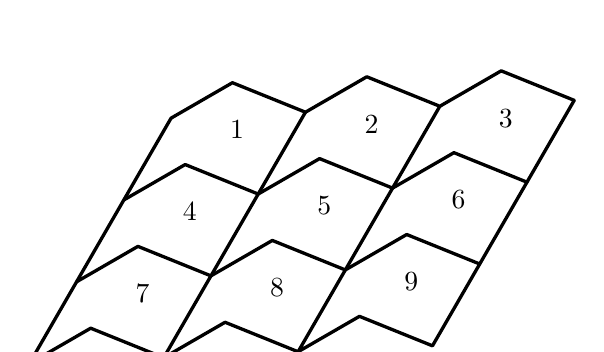
\begin{tikzpicture}[line cap=round, line join=round,baseline={(current bounding box.center)}]
	\newcounter{motif}
	\setcounter{motif}{6}
	\draw[line width=1.2pt]
		 (0,0)--++(60:3.6)
		 (0,0)++(30:0.9)++(-22:1)--++(60:3.6)
		 (0,0)++(30:0.9)++(-22:1)++(30:0.9)++(-22:1)--++(60:3.6)
		 (0,0)--++(30:0.9)--++(-22:1)--++(30:0.9)--++(-22:1)--++(30:0.9)--++(-22:1)--++(60:3.6)  ;
	\foreach \j in {1,2,3}
		{\draw[line width=1.2pt,shift={(60:\j*1.2)}] (0,0)--++(30:0.9)node[below=3.5mm]{\stepcounter{motif} \no \themotif} -- ++(-22:1)-- ++(30:0.9)node[below=3.5mm]{\stepcounter{motif} \no \themotif} --++(-22:1)--
		++(30:0.9)node[below=3.5mm]{\stepcounter{motif} \no \themotif \addtocounter{motif}{-6}} --++(-22:1)   ;}
\end{tikzpicture} \hfill~
%Fin tikz

\subsection*{Question 3}

Une boîte opaque contient 3 boules rouges et 5 boules vertes identiques et indiscernables au toucher. On pioche une boule au hasard.

Quelle est la probabilité qu'elle soit rouge ?

\medskip

\begin{minipage}{0.63\linewidth}
\subsection*{Question 4}
Recopier sur la copie et compléter avec des longueurs des côtés du triangle JLK pour que l'égalité ci-dessous soit vraie.

\[\cos\left(\widehat{\mathrm{LKJ}}\right) = \dfrac{\dots}{\dots}\]
\end{minipage}\hfill
%%Début PSTricks
%\begin{minipage}{0.30\linewidth}
%\psset{unit=1cm}
%\begin{center}
%	\begin{pspicture}(4.5,3.4)\
%		\pspolygon(0.2,0.8)(4.25,0.2)(2.2,2.5)%JKL
%		\uput[dl](0.2,0.8){J} \uput[dr](4.25,0.2){K} \uput[u](2.2,2.5){L}
%		\rput{-137}(2.2,2.5){\psframe(0.25,0.25)}\psarc(4.25,0.2){0.7}{129}{170}
%	\end{pspicture}
%\end{center}
%\end{minipage}
%%fin PSTricks
%Début Tikz
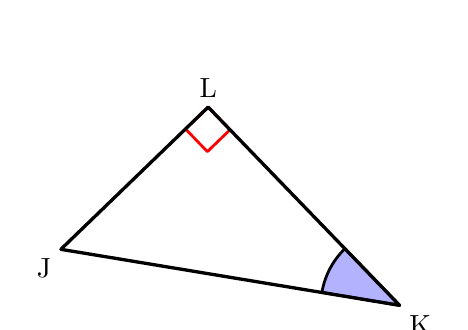
\begin{tikzpicture}[rotate=-46,line cap=round, line join=round,baseline={(current bounding box.center)}]
\coordinate (L) at (0,0);
\coordinate (K) at (3.5,0);
\coordinate (J) at (0,-2.6);
\draw[line width=1pt,red] (0,0) rectangle (0.4,-0.4) ;
\draw[line width=1pt,fill=blue!30,shift={(3.5,0)}] (0,0) --(-1,0) arc (180:216.5:1)--cycle ;
\draw[line width=1.2pt] (J) -- (K) -- (L) -- cycle;
\node[below left] at (J) {J};
\node[below right] at (K) {K};
\node[above] at (L) {L};
\end{tikzpicture}
%Fin Tikz

\subsection*{Question 5}

La distance entre la Terre et Mars est environ égale à \np{311200000}~kilomètres.

Donner la notation scientifique de \np{311200000}.

\subsection*{Question 6}

Charlie a effectué un trajet en vélo en 2~h 30~min à une vitesse moyenne de 40 km/h.

Calculer la distance, en km, parcourue par Charlie.

\subsection*{Question 7}
Recopier sur la copie la forme factorisée de l'expression $5x + 5$.

\begin{center}
\begin{tblr}{*{4}{|X[c]}|}\hline
	$5(x+1)$ & $5(x+5)$ & $10x$ & $25x$ \\
	\hline
\end{tblr}
\end{center}

\subsection*{Question 8}
Un article coûte 80~\euro. Son prix baisse de 10\,\%. Recopier sur la copie le calcul permettant de trouver le prix final de l'article.

\begin{center}
\begin{tblr}{*{4}{|X[c]}|}
	\hline
	$80 - 10$ & $80 - \dfrac{10}{100}$ & $80 - \dfrac{10}{100} \times 80$ & $\left(80 - \dfrac{10}{100}\right) \times 80$ \\
	\hline
\end{tblr}
\end{center}

\subsection*{Question 9}
Le graphique suivant donne la hauteur d'eau dans le port de Quiberon le 23 juillet 2025.

%Début Tikz
\begin{center}
		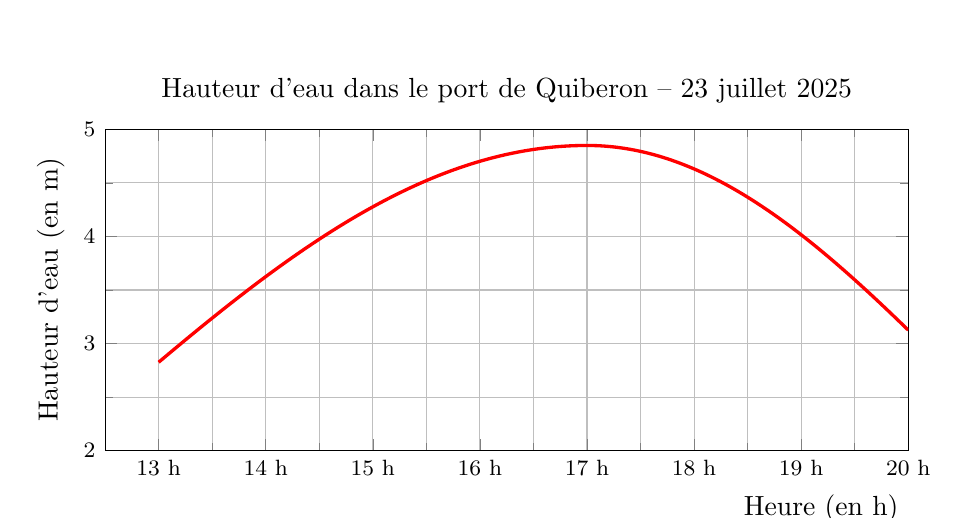
\begin{tikzpicture}%compiler avec pgfplots
			\begin{axis}[/pgf/number format/.cd, use comma,
				title style = {align = center},
				title={Hauteur d'eau dans le port de Quiberon  -- 23 juillet 2025},
				xlabel={Heure (en h)},
		 		xlabel style={
					at={(ticklabel cs:1)},
					anchor=north east},
				ylabel={Hauteur d'eau (en m)},
				x={13.6mm}, y={13.6mm},
				xmin = 12.5, xmax = 20,
				ymin = 2, ymax = 5,
				xtick = {13,14,15,16,17,18,19,20},
				xticklabels = {13~h, 14~h, 15~h, 16~h, 17~h, 18~h, 19~h, 20~h},
				ytick distance=1,
				tick label style={font=\footnotesize},
				minor tick num = 1,
				grid=both]
				\addplot [line width=1.2pt,color=red,smooth,samples=100,domain= 17:20 ]{2.6 + 2.25*cos((x-17)*25.5)};
				\addplot [line width=1.2pt,color=red,smooth,samples=100,domain= 13:17 ]{2.4 + 2.45*cos((x-17)*20)};
			\end{axis}
		\end{tikzpicture}
\end{center}
%Fin Tikz
%%PSTricks
%\medskip
%\begin{center}
%\psset{unit=1.25cm}
%\begin{pspicture}(-1,-1)(8.5,4)
%	\psaxes[linewidth=1.25pt,Ox=12,Oy=2,labelFontSize=\scriptstyle](0,0)(0,0)(7.5,3)
%	\multido{\n=0.0+0.5}{17}{\psline[linewidth=0.15pt](\n,0)(\n,3)}
%	\multido{\n=0.0+0.5}{7}{\psline[linewidth=0.15pt](0,\n)(8,\n)}
%	\pscspline[linecolor=blue,linewidth=1.25pt](1,0.7)(2,1.55)(3,2.3)(4,2.7)(5,2.8)(6,2.65)(7,2.05)(8,1.15)
%	\rput(3.75,3.4){\small 23 juillet 2025}
%	\rput(3.75,3.75){\small Hauteur d'eau dans le port de Quiberon}
%	\uput[u](7.5,0){\small Heure (en h)}
%	\rput{90}(-0.7,1.5){\small Hauteur d'eau (en m)}
%\end{pspicture}
%\end{center}
%%Fin PSTricks

Avec la précision permise par le graphique, recopier sur la copie la durée pendant laquelle la hauteur d'eau dans le port a été supérieure à 4 m.

\begin{center}
\begin{tblr}{*{4}{|X[c]}|}\hline
	2 h 30 min & 4 h 30 min & 5 h 30 min & 7 h \\ \hline
\end{tblr}
\end{center}

\begin{center}
\emph{Restitution de la copie du candidat à l'issue de la partie 1}
\end{center}

\newpage
\section*{\centering DEUXIÈME PARTIE (14 pts)}

\begin{quote}
\emph{Dans cette partie, toutes les réponses doivent être justifiées, sauf si une indication contraire est donnée.\\
	La clarté et la précision des raisonnements ainsi que la rédaction sont évaluées sur 2 points.\\
	Pour chaque question, si le travail n'est pas terminé, laisser tout de même une trace de la recherche ; les essais et les démarches engagées, même non aboutis, seront pris en compte dans la notation.}
	\end{quote}

\needspace{10\baselineskip}
\section*{Exercice 1 \hfill 4 points}

	Dans cet exercice, on considère la figure ci-contre.

	\medskip

	\begin{minipage}{0.47\linewidth}
Les points A, B et M sont alignés.

Les points A, C et N sont alignés.

Le triangle ABC est rectangle en B.

Le triangle AMN est rectangle en M.
\end{minipage}\hfill
%%début PSTricks
%\begin{minipage}{0.49\linewidth}
%\psset{unit=1cm,arrowsize=2pt 3}
%\begin{pspicture}(7,4.8)
%	%\psgrid
%	\psline(0,0.6)(7,4.7)
%	\psline(1,1.2)(6,1.2)(6,4.1)%AMN
%	\psline(4,1.2)(4,2.96)%BC
%	\uput[dl](1,1.2){A} \uput[r](6,1.2){M} \uput[dr](6,4.1){N}
%	\uput[ur](4,1.2){B} \uput[ur](3.9,3.13){C}
%	\psline[linewidth=0.8pt]{<->}(1,0.8)(4,0.8)\uput[d](2.5,0.8){6,4 cm}
%	\psline[linewidth=0.8pt]{<->}(4,0.8)(6,0.8)\uput[d](5,0.8){3,2 cm}
%	\psline[linewidth=0.8pt]{<->}(0.9,1.3)(3.95,3.11)\rput{31}(2.5,2.45){8 cm}
%	\psframe(4,1.2)(3.75,1.45)
%	\psline(6,1.2)(6,0)%M..
%\end{pspicture}
%\end{minipage}
%%Fin PSTricks
%Tikz
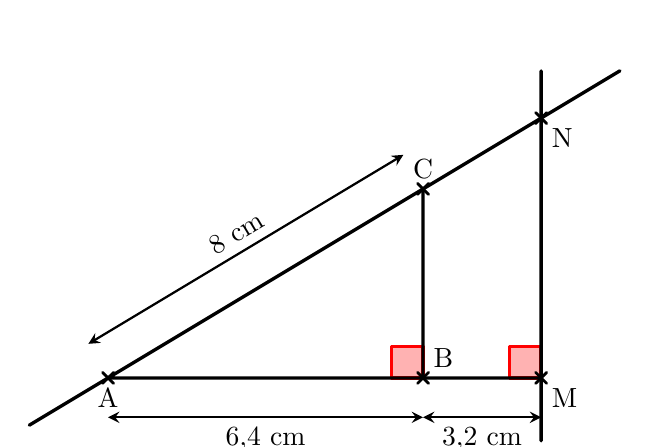
\begin{tikzpicture}[baseline={(current bounding box.center)},line join=round, line cap=round]
\coordinate (A) at (0,0);
\coordinate (B) at (4,0);
\coordinate (M) at (5.5,0);
\coordinate (C) at (4,2.4);
\coordinate (N) at (5.5,3.3);
\draw[line width=1.2pt,red,fill=red!30] (4,0) rectangle ++(-0.4,0.4)
 	(5.5,0) rectangle ++(-0.4,0.4) ;
\draw[line width=1.2pt]
	(A) -- (M)
	(B) -- (C)
	(-1,-0.6) -- (6.5,3.9)
	(5.5,-0.8) -- (5.5,3.9);
\foreach \coor/\nom/\pos in {(A)/A/below, (B)/B/{above right},
	(C)/C/above, (M)/M/{below right}, (N)/N/{below right}}
	{\draw[line width=1pt, shift={\coor}] (2pt,2pt)--(-2pt,-2pt) (2pt,-2pt)--(-2pt,2pt) (0,0) node[\pos]{\nom} ;}
	\draw[<->, line width=0.8pt, > = stealth,shift={(0,-0.5)}] (0,0) -- (4,0) node[pos=0.5,below,sloped]{6,4 cm} ;
	\draw[<->, line width=0.8pt, > = stealth,shift={(0,-0.5)}] (5.5,0) -- (4,0) node[pos=0.5,below,sloped]{3,2 cm} ;
	\draw[<->, line width=0.8pt, > = stealth,shift={(120:0.5)}] (0,0) -- (4,2.4) node[pos=0.5,above,sloped]{8 cm} ;
\end{tikzpicture}\hfill~
%Fin tikz


\medskip

On donne :

AB $= 6,4$ cm ; BM $= 3,2$ cm et AC $= 8$ cm.

\emph{La figure n'est pas en vraie grandeur.}

\begin{enumerate}
\item Tracer sur la copie le triangle ABC en vraie grandeur et en laissant les traits de construction.
\item Démontrer que BC $= 4,8$ cm.
\item Justifier que les droites (BC) et (MN) sont parallèles.
\item Démontrer que MN $= 7,2$ cm et AN $= 12$ cm.
\item Le périmètre du triangle ABC et le périmètre du quadrilatère BMNC sont-ils égaux ?\\
\textbf{Argumenter la réponse en précisant la démarche.}
\end{enumerate}

\needspace{10\baselineskip}
\section*{Exercice 2 \hfill 3,5 points}

\emph{Les deux parties de l'exercice sont indépendantes.}

\subsection*{Partie A}

Une confiserie fabrique des bonbons multicolores au goût réglisse. Ces bonbons de longueur totale 15 mm ont la forme de gélules constituées de trois parties : un cylindre et deux demi-boules identiques de rayon $R = 2{,}5$ mm comme le montre le schéma ci-dessous.

\begin{minipage}{0.48\linewidth}
%%Début Tikz
\begin{center}
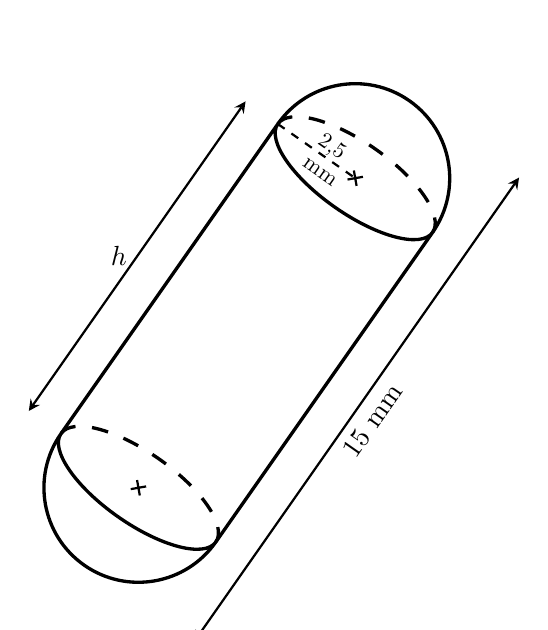
\begin{tikzpicture}[rotate=-35]
 \draw[line width=1.2pt] (-1.2,4.8) arc(180:0:1.2)--(1.2,0) arc (0:-180:1.2) -- cycle
 (-1.2,4.8) arc(-180:0:1.2 and 0.45)
 (-1.2,0) arc(-180:0:1.2 and 0.45);
 \draw[line width=1.2pt,dash pattern=on 6pt off 6pt]
 (-1.2,4.8) arc(180:0:1.2 and 0.45)
 (-1.2,0) arc(180:0:1.2 and 0.45);
 \draw[line width=0.8pt,dash pattern=on 3pt off 3pt]
 (-1.2,4.8) -- (0,4.8) node[pos=0.5,text width=1.2mm, align=center,rotate=-35,scale=0.8]{2,5 mm};
 \draw[<->, line width=0.8pt, > = stealth,shift={(-0.5,0)}] (-1.2,0)--(-1.2,4.8) node[pos=0.5,left]{$h$};
 \draw[<->, line width=0.8pt, > = stealth,shift={(0.5,0)}] (1.2,-1.2)--(1.2,6) node[pos=0.5,below, sloped,rotate=-35]{15 mm};
 \draw[line width=0.8pt] (-2pt,-2pt)--(2pt,2pt) (-2pt,2pt)--(2pt,-2pt);
 \draw[line width=0.8pt,shift={(0,4.8)}] (-2pt,-2pt)--(2pt,2pt) (-2pt,2pt)--(2pt,-2pt);
\end{tikzpicture}
\end{center}
%%Fin Tikz
%%%Début PSTricks
%\psset{unit=1cm,arrowsize=2pt 3}
%\begin{pspicture}(-2,-1.5)(2,6)
%	\psellipticarc(0,0)(1.1,0.4){180}{360}
%	\psellipticarc[linestyle=dashed](0,0)(1.1,0.4){0}{180}
%	\psarc(0,0){1.1}{180}{360}
%	\psline(1.1,0)(1.1,4.7)
%	\psline(-1.1,0)(-1.1,4.7)
%	\psellipticarc(0,4.7)(1.1,0.4){180}{360}
%	\psellipticarc[linestyle=dashed](0,4.7)(1.1,0.4){0}{180}
%	\psarc(0,4.7){1.1}{0}{180}
%	\psline[linewidth=0.8pt]{<->}(-1.5,0)(-1.5,4.7)\uput[l](-1.5,2.35){$h$}
%	\psline[linewidth=0.8pt]{<->}(1.5,-1.1)(1.5,5.8)\rput{90}(1.8,2.35){15 mm}
%	\psdots[dotstyle=+,dotangle=45](0,0)(0,4.7)
%	\psline[linestyle=dashed](0,4.7)(-1.1,4.7)\uput[u](-0.55,4.7){\footnotesize 2,5 mm}
%\end{pspicture}
%%%Fin PSTricks
%\emph{(Gélule : cylindre de hauteur $h$ flanqué de deux demi-sphères de rayon $2,5$ mm ; longueur totale $15$ mm.)}
\end{minipage}\hfill
\fbox{
	\begin{minipage}{0.4\textwidth}
	\textbf{Rappels}

	\begin{itemize}
		\item Volume d'un cylindre de rayon $R$ et de hauteur $h$ :
		\[ V = \pi \times R^2 \times h \]

		\item Volume d'une boule de rayon $R$ :
		\[ V = \frac{4}{3} \times \pi \times R^3 \]

		\item $1\text{ L} = 1\text{ dm}^3$
	\end{itemize}
\end{minipage}}\hfill~

\begin{enumerate}
	\item Montrer que la hauteur $h$ du cylindre est égale à $10$ mm.
	\item \begin{enumerate}
		\item Montrer que le volume de la partie cylindrique d'un bonbon est environ égal à $196$ mm$^3$.
		\item Léa affirme que le volume total d'un bonbon est compris entre $260$ et $262$ mm$^3$.

		A-t-elle raison ?
	\end{enumerate}
	\item Pour réaliser ces bonbons, la confiserie fabrique un mélange d'ingrédients qui est chauffé puis versé dans des moules en forme de gélule avant d'être refroidi.

	La confiserie fabrique chaque jour $83$L de mélange.

	Avec cette quantité de mélange, peut-elle produire plus de \np{300000} bonbons par jour ?
\end{enumerate}

\subsection*{Partie B}

Dans un magasin, les bonbons sont vendus en deux formats possibles :

\medskip
	\begin{tblr}{colspec={|X[c]|X[c]|},row{1}={font=\bfseries,cmd={\underline}}}
		\hline
		Format A          & Format B          \\
		Sachet de 500 g de bonbons & Sachet de 250 g de bonbons \\
		7,90~\euro{} le sachet     & 4,30~\euro{} le sachet     \\
		                           & \emph{\textbf{Offre promotionnelle} : pour 3 sachets achetés, le quatrième est à moitié prix.} \\ \hline
	\end{tblr}

\medskip
Léa veut acheter 1 kg de bonbons.

Quel format doit-elle choisir pour payer le moins cher possible ? \textbf{Argumenter la réponse en précisant la démarche.}

\needspace{10\baselineskip}
\section*{Exercice 3 \hfill 4,5 points}

Voici deux programmes de calcul :

\begin{center}
	\begin{minipage}{0.48\textwidth}
		\centering \textbf{Programme A}

		\begin{center}
			%Début Tikz
			\usetikzlibrary{positioning}
			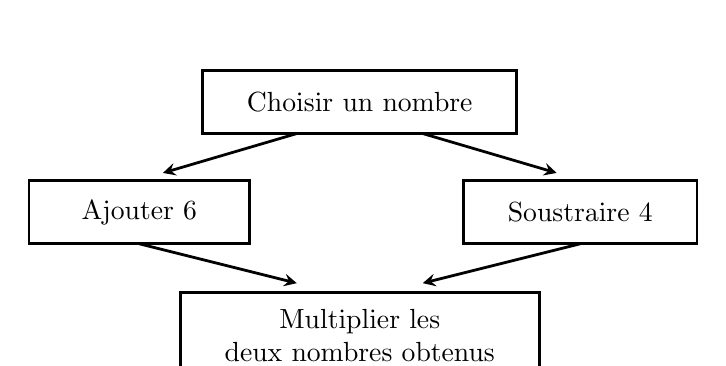
\begin{tikzpicture}[every node/.style={draw,line width=1pt, fill=white, align=center, rectangle, inner xsep=16pt, inner ysep=6pt, minimum width=2.8cm,minimum height=8mm},> = stealth]
				\draw[->,line width=1pt] (-0.8,-0.4) -- (-2.5,-0.9);
				\draw[->,line width=1pt] (0.8,-0.4) -- (2.5,-0.9);
				\draw[->,line width=1pt] (-2.8,-1.8) -- (-0.8,-2.3);
				\draw[->,line width=1pt] ( 2.8,-1.8) -- ( 0.8,-2.3);
				\node at(0,0) {Choisir un nombre};
				\node at (-2.8,-1.4) {Ajouter 6};
				\node at (2.8,-1.4) {Soustraire 4};
				\node[below] at (0,-2.4) {Multiplier les\\deux nombres obtenus};

			\end{tikzpicture}
			%Fin Tikz
%			%Début PSTricks
%			\psset{unit=1cm,arrowsize=2pt 3}
%			\begin{pspicture}(-3.5,0)(3.5,4)
%				\rput(0,3.5){\fbox{Choisir un nombre}}\psline{->}(-0.6,3.2)(-2.1,2.5)
%				\rput(-2,2.2){\fbox{Ajouter 6}}
%				\rput(2,2.2){\fbox{Soustraire 4}}\psline{->}(0.8,3.2)(2,2.5)
%				\rput(0,0.9){Multiplier les}\psline{->}(-2,1.9)(-0.8,1.1)
%				\rput(0,0.6){deux nombres obtenus}\psline{->}(2,1.9)(0.8,1.1)
%				\psframe(-2,0.4)(2,1.1)
%			\end{pspicture}
%			%Fin PSTricks
		\end{center}
	\end{minipage}
	\hfill
	\begin{minipage}{0.48\textwidth}
		\centering \textbf{Programme B}\\[0.3em]
		\begin{flushleft}
			\textbullet~\ Choisir un nombre.\\
			\textbullet~\ Calculer le carré de ce nombre.\\
			\textbullet~\ Soustraire 9.
		\end{flushleft}
	\end{minipage}
\end{center}

\begin{enumerate}
	\item On choisit 1 comme nombre de départ. Vérifier que le résultat obtenu avec le programme A est $- 21$.
	\item On choisit 10 comme nombre de départ. Calculer le résultat obtenu avec le programme B.
	\item Donner tous les nombres de départ possibles qui permettent d'obtenir 16 avec le programme B.
	\item \begin{minipage}[t]{0.35\linewidth}
		\textbf{(Question algorithmique)}

		Le programme ci-contre a été conçu avec le logiciel Scratch.

		Recopier et compléter sur la copie les lignes 3, 4 et 5 pour qu'il affiche le résultat obtenu avec le programme A lorsqu'un nombre de départ est saisi.

		\emph{Aucune justification n'est attendue.}
	\end{minipage}\hfill
		\begin{scratch}[scale=0.9,num blocks]
			\blockinit{Quand \greenflag est cliqué}
			\blocksensing{demander \ovalnum{choisir un nombre} et attendre}
			\blockvariable{mettre \selectmenu{Valeur 1} à \ovaloperator{\ovalvariable{réponse} + \ovalnum{}}}
			\blockvariable{mettre \selectmenu{Valeur 2} à \ovaloperator{\ovalvariable{réponse} - \ovalnum{}}}
			\blockvariable{mettre \selectmenu{Résultat} à \ovalnum{} * \ovalnum{}}
			\blocklook{dire \ovaloperator{regrouper\ovalnum{ Le résultat du programme A est} et {\ovalvariable{Résultat}}}}
		\end{scratch}
	%\begin{tabular}{|c|l|}
	%\hline
	%1 & Quand [drapeau vert] est cliqué \\
	%2 & demander \texttt{(Choisir un nombre)} et attendre \\
	%3 & mettre \texttt{Valeur 1} à \texttt{(réponse) + ( \ \ )} \\
	%4 & mettre \texttt{Valeur 2} à \texttt{(réponse) -- ( \ \ )} \\
	%5 & mettre \texttt{Résultat} à \texttt{( \ \ ) * ( \ \ )} \\
	%6 & dire \texttt{(regrouper(Le résultat du programme A est) et (Résultat))} \\
	%\hline
	%\end{tabular}
	%
	%\emph{(Lignes 3, 4 et 5 à compléter par le candidat avec les valeurs manquantes.)}

	\item On choisit $x$ comme nombre de départ. Montrer que le résultat obtenu avec le programme A est $x^2 + 2x - 24$.
	\item On cherche quel nombre de départ choisir pour que les programmes A et B donnent le même résultat. Écrire une équation permettant d'obtenir ce nombre de départ, puis la résoudre.
\end{enumerate}
\end{document}